\section{Predição no lado do cliente}
\label{sec:client_side_prediction}

No contexto de videogames, alguns gêneros possuem problemas semelhantes aos que os ambientes musicais enfrentam. Aqueles que utilizam reações como uma das mecânicas de \textit{gameplay}, como luta e FPS (\textit{first-person shooter}), para implementar funcionalidades \textit{online}, necessitam que haja pouco atraso entre os \textit{inputs} dos jogadores.

Há duas vertentes de implementação de jogabilidade \textit{online} em videogames - (1) \textit{Delay-based} ("baseado em atraso")\cite{rollback} e (2) \textit{Client-side prediction} ("Predição no lado do cliente", popularmente conhecido como \textit{Rollback Netcode})\cite{client-side-prediction}.

\subsection{\textit{Delay-based}}

Nessa abordagem, todos os \textit{inputs} dos transmissores são esperados antes que as ações correspondentes possam ser executadas \cite{rollback}. Essa implementação é trivial e garante a corretude dos dados transmitidos; no entanto, para conexões de alta latência, nas quais o tempo de transmissão via Internet seja maior que o tempo mínimo de ação local, os jogadores terão uma sensação de "lentidão".

Esse limite máximo de latência varia a cada jogo. Para oferecerem uma experiência fluida, de acordo com o tempo de reação à estímulos visuais, é esperado que não haja mais que 100 ms de atraso entre as ações dos jogadores \cite{pubnub}. Esse limite, no entanto, é apenas uma estimativa - idealmente, a melhor implementação deve garantir que não haja diferença entre jogar \textit{online} ou localmente. Esse limite dependerá de especificações de cada jogo, como FPS (\textit{frame-per-second}) e a latência natural causada pelo dispositivo de controle (\textit{input delay}). Desenvolvedores também podem adicionar um atraso artificial, para aumentar a tolerância de tempo causado pela transmissão dos pacotes via Internet.

No contexto de ambientes musicais \textit{online}, podemos comparar esse método com as soluções síncronas citadas na \secref{sec:delay-based-audio-solutions}. Nesses casos, assim como presente no contexto de videogames, essa técnica é muito sensível à latência causada pela transmissão de pacotes via Internet entre os participantes. As soluções citadas, portanto, focam em reduzir o tempo total de transmissão, mas são limitadas por fatores externos, exigindo bandas de alta velocidade e/ou proximidade geográfica.

\subsection{\textit{Client-side prediction}}

A implementação do \textit{Client-side prediction} (\figref{fig:rollback_diagram}), por outro lado, aumenta a tolerância da espera dos pacotes propondo a previsão dos \textit{inputs} dos jogadores antes que cheguem via Internet utilizando dados já recebidos anteriormente. Caso as previsões sejam incorretas, o estado de jogo no momento em que a previsão foi realizado é retornado, portanto, o nome popular "\textit{rollback}" (reversão) \cite{rollback}.

\begin{figure}[htbp]
\centering
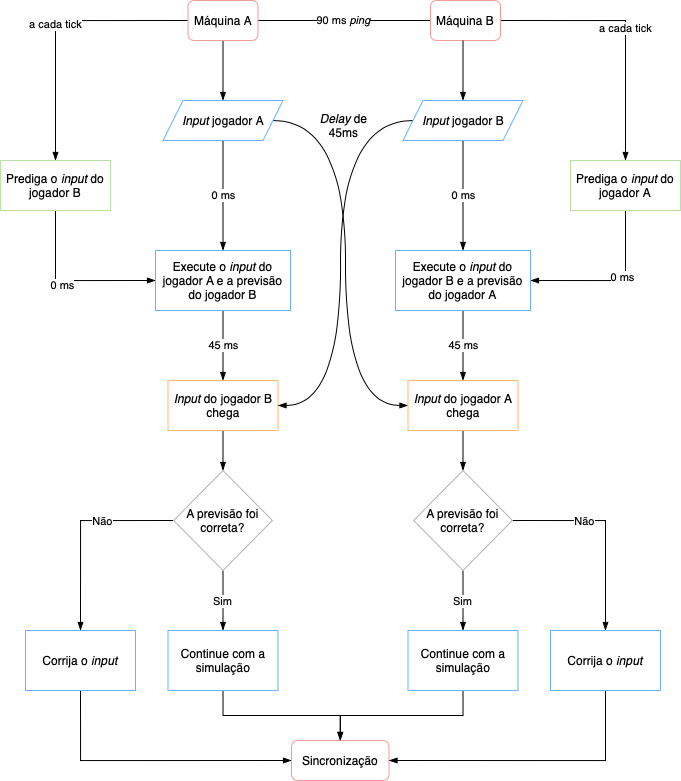
\includegraphics[width=1\textwidth]{images/rollback.png}
\caption{Diagrama demonstrando o processo de execução e sincronização dos \textit{inputs} de dois jogadores (com \textit{ping} de 90 ms entre eles) em um jogo \textit{online} utilizando \textit{client-side prediction} em um modelo \textit{peer-to-peer}. Tradução da imagem criada por GerardSN, CC BY-SA 4.0, https://commons.wikimedia.org/w/index.php?curid=97477279.}
\label{fig:rollback_diagram}
\end{figure}

A necessidade da implementação do \textit{client-side prediction} surge em 1996, em um contexto onde a maioria dos usuários de Internet possuíam conexões discadas com banda entre 28 Kb/s e 34 Kb/s \cite{broadband}. \textit{Duke Nukem 3D}, um jogo do gênero FPS (\textit{first-person shooter}, "tiro em primeira pessoa), foi pioneiro na utilização desse algoritmo para prover sincronia entre os jogadores \textit{online} \cite{duke_nukem}, que podem possuir diferentes velocidades de Internet ou estarem distantes entre si. Os \textit{inputs} dos jogadores remotos eram previstos no lado do cliente e enviados a um servidor central, que comparava os \textit{inputs} corretos e enviava as correções necessárias.

O modelo de previsão, isto é, o algoritmo utilizado para prever os \textit{inputs} dos jogadores remotos, pode variar de acordo com as necessidades específicas dos jogos. O modelo proposto por Bernier, utilizado no jogo \textit{Half-Life}, apenas repete os últimos \textit{inputs} reconhecidos pelo servidor \cite{client-side-prediction}. Este modelo assume que os \textit{inputs} tendem a se repetir com frequência a cada \textit{frame}, portanto, apenas repeti-los e corrigir aqueles que não se enquadram funcionam para a maioria dos casos.

A utilização de \textit{client-side prediction} expande-se para diferentes gêneros, como o de luta, e sua adoção é vista positivamente pelos jogadores \cite{rollback_success}. Por não necessitar esperar os \textit{inputs} dos adversários para execução do jogador localmente, a sensação de fluidez é mais atingível.

No entanto, por não garantir a corretude dos \textit{inputs} imediatamente após a previsão, é necessário haver a correção do estado do jogo. Essa correção pode causar, por exemplo, que um jogador perceba que seu adversário está em uma posição no espaço e, em outro momento, mudar de lugar instantaneamente, causando uma sensação de "teletransporte". Fatores como \textit{FPS} (\textit{frames per second}, "quadros renderizados por segundo") e a latência entre os jogadores, que não são valores constantes, desafiam os desenvolvedores a manter a sincronia entre todos os clientes \cite{client-side-prediction}.